% The Flower: visualizing the solved-move landscape of the rank-48
% 4x4 scheme.  Build: tectonic doc/matmul_flower_paper.tex
\documentclass[10pt]{article}
\usepackage[margin=2.4cm]{geometry}
\usepackage{amsmath,amssymb}
\usepackage{booktabs}
\usepackage{graphicx}
\usepackage{fancyvrb}
\usepackage{enumitem}
\usepackage{microtype}
\usepackage[hidelinks]{hyperref}
\urlstyle{same}
\setlist{itemsep=2pt,topsep=3pt}
\setlength{\emergencystretch}{3em}
\DefineVerbatimEnvironment{Code}{Verbatim}{fontsize=\footnotesize}

\title{\bfseries The Flower: Visualizing the Solved-Move Landscape of
  the Rank-48 $4\times4$ Scheme, and the Search Heuristics It Yields}
\author{Greg Sidebottom}
\date{}

\begin{document}
\maketitle
\vspace{-3em}
\begin{center}
\itshape Research note --- logic repo
(\url{https://github.com/gsidebottom/logic}), matmul track,
2026-07-09. Companion to ``Rigidity of the Rank-48 $4\times4$
Matrix-Multiplication Scheme under Solved Flip Moves''
(\texttt{doc/matmul\_rigid48\_paper.md}), which proves the theorem
this note visualizes, and to the $3\times3$ additive-complexity paper
(\texttt{doc/matmul\_adds\_paper.md}). Interactive version of
Figure~\ref{fig:flower}:
\path{https://claude.ai/code/artifact/e2167bb4-fb0d-4295-a0f9-b4554142e39d}.
Every number below has a mechanical check (\S\ref{sec:repro}).
\end{center}

\section*{Abstract}

The companion paper proves that the rational rank-48 scheme for
$4\times4$ matrix multiplication --- the only rank-48 scheme usable
over the real numbers --- is \emph{rigid}: the graph of states
reachable by one split and solved flips is finite (7{,}408 states) and
contains no reduction except the trivial return to the seed. This
note treats that certified graph as \textbf{data}. We export it with
per-state search metrics, visualize it, and read off its anatomy,
which turns out to be strikingly simple: a \textbf{flower} --- a
single hub (the seed), 6{,}488 pendant leaves that admit no move
except undoing themselves, and a thin 920-state \emph{fringe} where
all nontrivial structure lives and where every local search signal
saturates almost immediately.

From the picture we derive five concrete search heuristics, and they
pay off at once: a gradient signal (\textbf{nearmiss}, the number of
solvable one-move coincidence targets) that is provably capped at 2
inside the certified component \textbf{deepens to 7 and then 14} one
split level further out, guiding a beam search; a $19\times$
budget-focusing rule; and a cost-recalibration discipline that caught
a uniform two-split enumeration mispriced by two orders of magnitude
(killed at 3\% after 18 CPU-hours; its true cost ${\approx}500$
CPU-hours) and replaced it with a guided program that covers the
region all metrics favor at a fraction of the price. Whether the
deepening gradient ever converts into an actual rank reduction --- a
new rank-48 scheme, or the characteristic-0 rank-47 that would be a
record --- is the open question the running campaigns address.

\section{The graph}\label{sec:graph}

All terms from the companion paper; briefly: the \textbf{seed} is the
Dumas--Pernet--Sedoglavic rational $\langle4\times4\times4:48\rangle$
decomposition (48 rank-one summands $a\otimes b\otimes c$ over
$\mathbb{Z}[\tfrac12]$); a \textbf{split} replaces a summand by two
(rank $+1$, and over $\mathbb{Q}$ can target \emph{any} partner's
factor); a \textbf{solved flip} is a flip whose scalar $\lambda$ is
chosen by solving $f_i+\lambda f_j=\mu f_m$ --- the only way exact
coincidences occur over the rationals; a \textbf{reduction} merges two
summands proportional in two slots (rank $-1$).

\texttt{flip48 --graph} exports the full 1-split component:
\textbf{7{,}409 nodes} (the seed plus 7{,}408 rank-49 states ---
independently matching the count pinned in the Lean theorem) and
\textbf{16{,}000 edges} (6{,}768 splits, 2{,}328 solved flips, 6{,}904
reductions), with four metrics per state:
\begin{itemize}
\item \textbf{shared} --- factor pairs equal in some slot (flip
  eligibility);
\item \textbf{coinc} --- solved flips available;
\item \textbf{nearmiss} --- distinct third summands reachable by a
  ply-1 coincidence: how many partners this state could become aligned
  with in one move. A reduction needs alignment with the \emph{same}
  partner in \emph{two} slots, so nearmiss counts the doors that a
  second aligned slot would turn into exits;
\item \textbf{copl} --- coplanar factor triples in the $a$-slot
  (rank-2 triples): the raw material from which solvable moves are
  made.
\end{itemize}

\section{Anatomy: the flower}\label{sec:anatomy}

\begin{figure}[t]
\centering
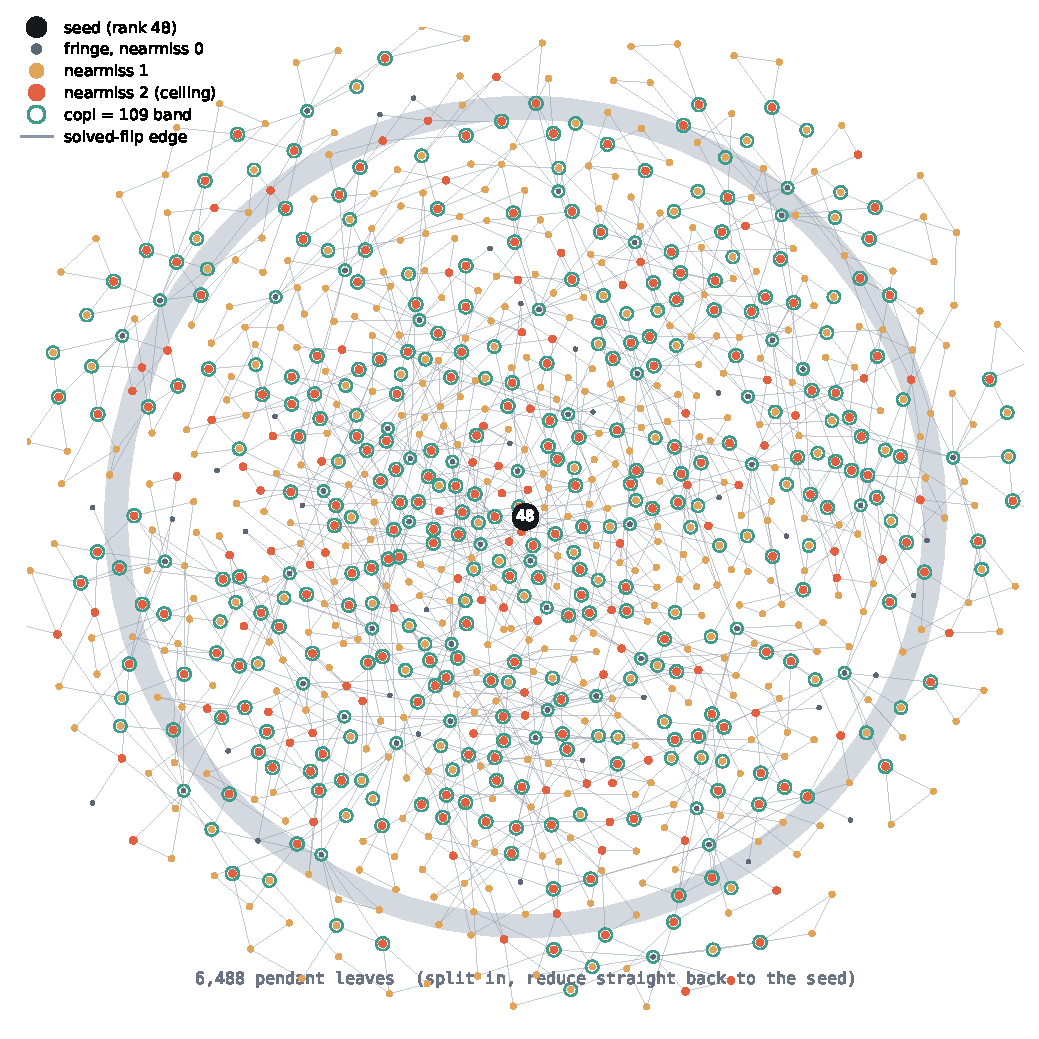
\includegraphics[width=.86\linewidth]{fig_flower.pdf}
\caption{The solved-move component. Hub $=$ seed; annulus $=$ 6{,}488
pendant leaves (aggregated); scattered structure $=$ the 920-state
flip-active fringe, colored by nearmiss, teal-ringed where
$\mathrm{copl}=109$.}
\label{fig:flower}
\end{figure}

\begin{center}
\begin{tabular}{@{}ll@{}}
\toprule
measurement & value\\
\midrule
states / edges & 7{,}409 / 16{,}000\\
reductions $\to$ seed & \textbf{6{,}904 of 6{,}904}\\
degree-2 pendant leaves & 6{,}488 (88\%)\\
flip-active fringe & 920 states, 1{,}468 flip edges\\
nearmiss distribution & 0: 6{,}568 \,$\cdot$\, 1: 516 \,$\cdot$\, 2: 324 --- \textbf{max 2}\\
coinc distribution & 0: 6{,}568 \,$\cdot$\, 2: 516 \,$\cdot$\, 4: 324\\
copl distribution & 63: 2{,}128 \,$\cdot$\, 64: 4{,}896 \,$\cdot$\, \textbf{109: 384}\\
max coefficient anywhere & 6 (magnitudes never grow)\\
\bottomrule
\end{tabular}
\end{center}

Three readings:
\begin{enumerate}
\item \textbf{The rigidity theorem, as one number.} Every one of the
  6{,}904 reduction edges points at the seed. The certified statement
  ``no reduction except the trivial return'' is \emph{visible}.
\item \textbf{The component is almost entirely inert.} 88\% of states
  are petals --- one move in, one move out, no interaction with
  anything. Uniform search effort is 88\% wasted by construction.
\item \textbf{The fringe is where structure lives, and its signals
  saturate.} Only 920 states have any solved flip at all; no state
  has more than 2 nearmiss targets or 4 available moves; and one
  distinguished band --- 384 states with 109 coplanar triples against
  the 63--64 baseline --- concentrates the geometric richness. Inside
  the certified component there is, quite literally, no gradient to
  climb: the landscape is flat at height 2.
\end{enumerate}

\section{The heuristics}\label{sec:heur}

\paragraph{H1 --- Spend search where the structure is ($19\times$
focusing).} Second splits from pendant leaves recreate the situation
the certificate already closed. Restricting second splits to the
920-state fringe (and ordering by nearmiss, then the copl-109 band)
concentrates the budget on ${\sim}12\%$ of parents with, empirically,
all of the signal.

\paragraph{H2 --- Never walk randomly; only solved moves.} (Restated
from the companion paper as an operating rule.) Ten million
random-$\lambda$ moves produced zero coincidences; exact events over
$\mathbb{Q}$ are measure-zero. Every productive move is the solution
of a small linear system --- search over $\mathbb{Q}$ is
\emph{constructive}, not stochastic.

\paragraph{H3 --- nearmiss is the gradient.} It measures exactly the
precondition of the goal event (a two-slot alignment with a single
partner). Its ceiling inside the certified component is 2; the
question ``is the landscape flat everywhere, or only here?'' is
decided by measuring it at depth. Measured: \textbf{depth-1 max 2
$\to$ sampled depth-2 max 7 $\to$ guided beam level-1 max 14 (mean
11.1 over a 1{,}500-state beam)}. The gradient is real, and it
steepens under guidance --- the strongest empirical argument yet that
the rigidity boundary is a property of the \emph{radius}, not of the
whole landscape.

\paragraph{H4 --- The copl band is a prior.} Coplanarity is the raw
material of solvable moves; the 384-state copl-109 band is the natural
first target for any deeper enumeration, and band membership is
computable before committing any search budget to a parent.

\paragraph{H5 --- Measure closure inflation before exhausting.} The
1-split closures average 2.3 states; a uniform 2-split enumeration
priced at that figure looked like a ${\sim}10$-CPU-hour job. Direct
measurement showed level-2 closures average \textbf{${\sim}580$ states
($250\times$)} --- repricing the uniform sweep at ${\sim}500$
CPU-hours. It was killed at 3\% (18 CPU-hours spent) and replaced with
the guided program below. The rule: before exhausting level $k{+}1$,
measure its branching on a sample; the extrapolation from level $k$ is
not a bound, it is a guess.

\section{The running program, and the open question}\label{sec:prog}

Two campaigns implement the heuristics (both with progress tickers,
global state budgets, and inline exact verification of any find):
\begin{itemize}
\item \textbf{Fringe-exhaustive} (\texttt{--pursue5 0 --fringe-only}):
  \emph{all} 7{,}056 second splits of each of the 840
  gradient-positive parents, every root closed under solved flips with
  reduction continuations. Zero findings here extends the rigidity
  certificate to ``no reduction reachable through the fringe at
  2-split radius.'' Status at writing: 200/840 parents (24\%),
  \textbf{1.24 billion states explored, zero reductions found}, and an
  independent confirmation of nearmiss-14 territory.
\item \textbf{Gradient chase} (\texttt{--pursue6}): best-first beam on
  nearmiss across split depths (beam 1{,}500, 60 sampled splits per
  frontier state). Level 1 complete: nearmiss max 14, mean 11.1. The
  chase asks the one question that matters: \textbf{does nearmiss keep
  climbing until a double-coincidence actually fires, or does it
  plateau --- and at what height?} A conversion produces a genuinely
  new rank-48 scheme (fresh material for the operation-count program
  of the companion papers) or a characteristic-0 rank-47 --- a record.
  A plateau maps the next rigidity boundary.
\end{itemize}

\section{Why visualize at all}\label{sec:why}

The honest answer: every quantitative decision in \S\ref{sec:heur}
was \emph{available} in raw logs, and none of it was \emph{seen} until
the graph was drawn. The flower shape --- hub, petals, thin fringe ---
made three facts simultaneously obvious that tables had kept separate:
reductions all point home; almost everything is inert; the interesting
minority is small enough to exhaust. One picture converted a mispriced
brute-force plan into a guided program and surfaced the gradient
question that is now the campaign's spine. For search spaces born from
exact algebra, where every state is expensive to think about
individually, a faithful picture of the \emph{whole} is the cheapest
instrument there is.

\section{Reproduction}\label{sec:repro}

\begin{Code}
cargo build --release --bin flip48
./target/release/flip48 --graph matmul/dps48/graph48.json --cap 256   # 17 s
# anatomy numbers: any JSON tool over graph48.json (see the table)
./target/release/flip48 --pursue5 0 --fringe-only --threads 8 \
    --budget 4000000000            # fringe-exhaustive campaign
./target/release/flip48 --pursue6 --beam 1500 --samples 60 --depth 8 \
    --threads 4                    # gradient chase
\end{Code}

The interactive Figure~\ref{fig:flower} (hover any fringe state for
its metrics) is published at the artifact URL in the front matter; the
static figure is regenerable from \texttt{graph48.json} by the script
in the repository history.

\section*{Acknowledgments}

This work was carried out in an extended interactive collaboration
with Claude (Anthropic; the Fable~5 and Opus~4.8 models), which
implemented the engines, the export and visualization, and much of
this text under the author's direction and review. Every number is
mechanically checkable via \S\ref{sec:repro}.

\section*{References}

\begin{itemize}
\item G. Sidebottom. \emph{Rigidity of the Rank-48 $4\times4$
  Matrix-Multiplication Scheme under Solved Flip Moves --- a
  Machine-Checked Obstruction.} Companion paper, this repository
  (2026).
\item G. Sidebottom. \emph{A 55-Addition Rank-23 Scheme for
  $3\times3$ Matrix Multiplication via Exact Two-Sided Minimization.}
  This repository (2026). Artifacts: DOI~\path{10.5281/zenodo.21240904}.
\item M. Kauers, J. Moosbauer. \emph{Flip Graphs for Matrix
  Multiplication.} arXiv:2212.01175 (2022).
\item J.-G. Dumas, C. Pernet, A. Sedoglavic. \emph{A Non-Commutative
  Algorithm for Multiplying $4\times4$ Matrices Using 48 Non-Complex
  Multiplications.} arXiv:2506.13242 (2025).
\item A. Novikov et al. \emph{AlphaEvolve: a Coding Agent for
  Scientific and Algorithmic Discovery.} arXiv:2506.13131 (2025).
\end{itemize}

\end{document}
